\documentclass{article}
\usepackage[margin=1in]{geometry}
\usepackage{amsmath}
\usepackage{xr}
\usepackage{xcolor}
\usepackage{siunitx}
\usepackage{gensymb}
\usepackage{graphicx}
\usepackage{wrapfig}
\usepackage{subcaption}
\usepackage{enumitem}
\usepackage{scrextend}
\usepackage[normalem]{ulem}
\usepackage{soul}

\externaldocument[S-]{Supporting_Information}
\externaldocument[M-]{Draft}

\begin{document}

\graphicspath{{./figures/}}

\begin{center}
\textbf{Response to reviewers: Statistical Inference of Transport Mechanisms and Long
        Time Scale Behavior from Time Series of Solute Trajectories in Nanostructured Membranes} \\
Authors: Benjamin J. Coscia, Christopher P. Calderon and Michael R. Shirts
\end{center}

We thank the reviewers for carefully reading over our manuscript and providing
thoughtful and constructive feedback. We have taken the suggestions into consideration 
and made appropriate revisions to the manuscript document. The comments have been reproduced
in italics and all changes to the text have been documented below them. Any newly added
references are given in the bibliography of this document and are placed in the main 
text with appropriate numbering.

\section*{Response to Reviewer 1}

\begin{enumerate}[label={Comment \theenumi :}, leftmargin=3.9\parindent]

    %r1_comment1
    \item \textit{The manuscript by Coscia et al. analyzes diffusion and transport of solute molecules
    in a low water content lyotropic liquid crystal using a statistical model developed on the basis 
    of molecular dynamics simulations. The purpose of the statistical model is two-fold; first to 
    extrapolate computed MSDs to longer times to obtain diffusion coefficients, and second to attempt
    to gain increased physical insight on diffusion mechanisms. These issues are important in 
    highly-confined/low-water content nanoporous materials, in which diffusion occurs through complex
    mechanisms and over long timescales. The manuscript will most likely be of interest to the community
    interested in nanoporous materials for separations.}
    
    Author reply: We thank the reviewer for their thoughtful assessment of our work.
    
    %r1_comment2
    \item \textit {Unfortunately, because there is no comparison with alternative techniques, it is 
    very difficult to evaluate this new approach relative to previous work that has examined similar 
    issues. There exist numerous other methods for extrapolating MSDs to longer time, which the 
    authors have not discussed. One such method is the “trajectory-extending kinetic Monte Carlo” 
    (TEKMC) approach of Brown and coworkers see e.g. Macromolecules 2010, 43, 9210-9214, 
    Macromolecules 2015, 48, 7346-7358, and J. Phys Chem. B, 2012, 116, 95-103. The authors should 
    add a comprehensive discussion of how their approach compares to this and similar methods. The 
    paper would be significantly improved if the authors were to perform and present TEKMC results 
    for their system, so that one could better evaluate the performance of their proposed method.}
    
    Author reply: We thank the reviewer for bringing our attention to these other interesting 
    approaches. They certainly merit discussion as alternative approaches for estimating mean 
    squared displacements on long timescales. We have added some discussion of these methods to 
    the introduction.
    
    \begin{quote}
    A number of approaches have been explored to inexpensively extend the relatively short
    trajectories output by molecular simulations which exhibit complex diffusive behaviors
    onto much longer timescales. The trajectory extending kinetic Monte Carlo (TEKMC) approach
    divides a unit cell into a three dimensional grid and quantifies the transition 
    probabilities of particles that can move between each subdivision allowing one to generate
    stochastic trajectories that reach the diffusive regime~\cite{neyertz_trajectory-extending_2010}
    If the dynamics of the system are fast enough, it is possible to parameterize TEKMC models with
    relatively short simulation trajectories which facilitates systematic studies of small perturbations
    to material constituents.~\cite{hanson_computer_2012}
    In a related approach, dynamic bond percolation (DBP) theory can be used to quantify the
    rate of transition between sites in a dynamically disordered medium and long timescale
    behavior can be propagated using kinetic Monte Carlo simulations.~\cite{druger_dynamic_1983}
    Webb et al. extended this approach by defining sites based on the molecular details of 
    a polymer electrolyte system, thus allowing them to explain ion diffusivities predicted by
    the model in terms of chemically specific interactions.~\cite{webb_chemically_2015}
    \end{quote} 
    
    We have also modified the first sentence of the paragraph that follows in order to maintain
    good flow.
    
    Original text:
    \begin{quote}
    We have already advanced our understanding of LLC monomer design in our previous work
    by building stochastic time series models based on the chemical intuition gained
    from qualitative MD studies of solute transport in an H\textsubscript{II} phase LLC
    membrane.
    \end{quote}
    
    Modified text:
    \begin{quote}
    Based on the chemical intuition gained from our previous qualitative MD studies of 
    solute transport in an H\textsubscript{II} phase LLC membrane, we have contributed our
    own stochastic modeling approaches with goals similar to both TEKMC and DBP.
    \end{quote}

    We agree that a full comparison of our method to other methods for computing long timescale 
    diffusion such as TEKMC would be very interesting and instructive but feel it would be better 
    suited as a separate study where we could evaluate a number of approaches, including perhaps
    recent approaches we have developed within our research group.~\cite{coscia_capturing_2020}
    It would be illuminating to test these methods on systems such as ours where there is
    a rich diversity of intermolecular interactions that work to immobilize solutes.
    Such a large-scale comparison would take more space and time than would be appropriate for 
    the current paper. Although methods such as TEKMC seems a fairly straightforward approach to
    implement, it is not immediately clear how we could optimally adapt the methodology to a 
    monoclinic unit cell with two dimensional order without in-depth testing.
    Regarding the CS-DBP model, we are not convinced it would be suitable for our goals because
    it relies on defining bound states and modeling hops between them. There are numerous potential
    locations within our LLC system where solutes can become bound in some way. The HDP-AR-HMM
    circumvents the need for relatively complicated methods used to identify binding sites 
    by automatically identifying distinct dynamics characteristic of classes of bound states. 
    
    As stated by the reviewer, there are two goals of our work: to obtain long timescale MSDs and
    to understand mechanisms leading to diffusive behavior. TEKMC may be a suitable alternative 
    approach to obtaining our first goal, but it is not clear that it could give the same level
    of mechanistic insight that the HDP-AR-HMM offers. Although the work by Hanson et al.
    (J. Phys Chem. B, 2012, 116, 95-103) is able to provide physical insight into the effect of
    nanoparticles on diffusion of gaseous penetrants in a polystyrene polymer matrix, it does so
    by testing hypotheses motivated by observations of the diffusion constant (predicted by TEKMC)
    in response to different temperatures and nanoparticle concentrations. This parallels well
    with the type of analysis we performed in our initial LLC transport work (J. Phys Chem. B, 2019, 123, 6314-6330)
    where we used the mean squared displacement and the qualitative characteristics of the solute
    time series in order to hypothesize transport mechanisms. In this work we ``re-discover" these
    mechanisms with minimal human intervention and characterize them in detail using the 
    HDP-AR-HMM while \textit{simultaneously} providing a method to estimate diffusion constants.

    \item \textit{Much of the writing seems more suitable for JCTC rather than JPC. I encourage the
    authors to better emphasize and discuss “new physical insight” and “chemical details”, and spend
    less time on methodology. For example pages 5-16 are all on methodology, yet it is not until 
    Figure 8 of the paper (page 26) that the authors give any description of what the LLC system 
    they are studying is actually composed of. Presumably the LLC is made up of self-assembled 
    monomers (in water) shown in Figure 8a). I would encourage the authors to describe their 
    system more concretely much earlier in the paper... there is also no information on system 
    size, box dimensions, etc.}
    
    Author reply: We thank the reviewer for encouraging us to include more physical insight and
    further details about our molecular simulations. We received feedback from the editor along 
    with these comments that the scope of JPC has been expanding, and that the methodological 
    details are appropriate. We have studied the structure of and transport of solutes within 
    this particular LLC system extensively in our previous work.~\cite{coscia_chemically_2019}
    We feel strongly that our current work should emphasize the HDP-AR-HMM as a more general 
    tool for understanding complex dynamics in systems beyond our example system. We would prefer
    not to cut any methodological details, as this would hurt the paper's reproducibility, and
    lengthening the paper by including additional physical insight may narrow the audience willing
    to dive in.
    
    We do agree that there are certain basic simulation details that we have neglected to 
    mention. Therefore we have made the following edits to section 2.1 of the methods:
    
    We added the highlighted text to the first sentence of the section:
    \begin{quote}
      We studied transport of solutes in the H\textsubscript{II} phase using \hl{our
      previously developed} atomistic molecular model of four pores in a 
      \hl{$9.4\times9.4\times7.6$ nm} monoclinic unit cell with 10\% water by weight, 
      \hl{totaling 62,000 atoms}.    
    \end{quote}
    
    We have also added the following text describing the model:
    \begin{quote}
    We modeled water molecules using the TIP3P water model,~\cite{jorgensen_comparison_1983}
    We used the Antechamber module shipped with AmberTools18 to parameterize monomers and 
    solutes using the Generalized Amber Force Field (GAFF).~\cite{wang_development_2004} We 
    assigned charges using the AM1-BCC model as implemented in Antechamber.~\cite{jakalian_fast_2000,jakalian_fast_2002}
    GAFF is very commonly used in simulations with diverse organic chemical functionality, 
    and was developed for consistency within the AMBER ecosystem, which uses TIP3P as the
    water model. We chose these standard force fields and generalizable parameterization 
    approaches so that a range of solutes and monomers could be self-consistently and easily 
    studied. The main goal of this work is to develop stochastic models which can reproduce
    solute behavior on MD time scales, independent of the choice of force field. In future 
    work, it may be beneficial to employ specialized force fields, including polarizable 
    force fields or other higher-order effects in order to improve the accuracy of structure 
    parameters and selectivity predictions.
    \end{quote}
    
    Finally, we have added a figure with a picture of the system which we are studying 
    (see Figure~\ref{fig:membrane_side_profile}).
    \begin{figure}
    \centering
    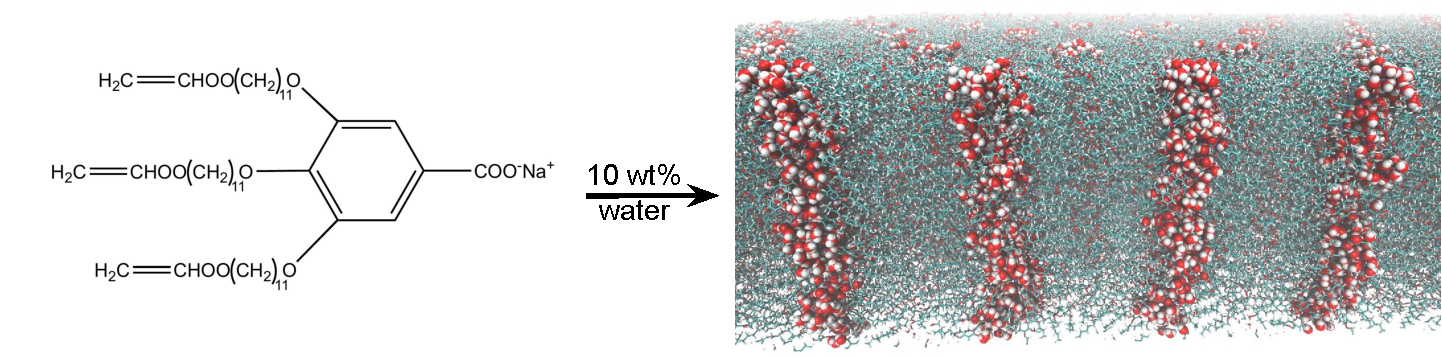
\includegraphics[width=\textwidth]{membrane_side_profile.pdf}
    \caption{When combined with 10 wt\% water, the LLC monomer studied in this work forms the 
    H\textsubscript{II} phase which is characterized by hexagonally packed columns with 
    hydrophilic pores. In the figure, white and red water molecules mark the membrane pores.
    The monomer fills the rest of the space. Note that water molecules are present in the 
    tails, but they are hidden for the sake of clarity. }\label{fig:membrane_side_profile}
    \end{figure}

    %r1_comment4
    \item \textit{The authors should more clearly note that their discussion largely applies only 
    to very low water content LLC regimes (such as the 10\% LLC studied). For higher water content 
    LLCs (e.g. $>$ 15-20\%) it is straightforward to obtain the diffusion limit from standard MD 
    simulations. While the authors are surely well aware of this, the reader may not be, and it is
    important to clearly distinguish the regimes.}
    
    Author reply: We thank the reviewer for making this point. In systems with less obstructions
    to motion, such as LLCs with a higher water content, most solutes and water will be 
    relatively unimpeded, and diffusion constants can be obtained by standard techniques.    
    However, we would still argue that our method would still be very useful for studying
    solute dynamics in these higher water content systems by allowing one to study the dynamics 
    of solutes that have longer residence times and interact with moieties in a complex medium. %portions of the system away from the pore center.
    %Interactions characterized by different dynamical behavior even on short time scales can
    %still be highly informative. 
    This is the basis for the point we make in the introduction:``. . . direct calculations 
    of diffusion constants may obscure the molecular mechanisms controlling transport". Therefore
    we would prefer not to limit the range of application of this method. 
    %BJC2: added    
    However, we do agree that it would be helpful to the reader to clarify that the level of modeling 
    which we present in this work is certainly not merited in cases where they are only interested in
    diffusion constants. Therefore, we have modified a paragraph in the introduction in order to
    encourage readers to pursue simpler approaches if the system allows it.
    
    Updated text with additions highlighted in yellow:
    
    \begin{quote}
    In this work, we are particularly interested in the design of lyotropic liquid 
    crystal (LLC) monomers, a class of amphiphilic molecules whose ordered self-assembled
    phases can be cross-linked into mechanically strong membranes capable of highly 
    selective separations. Inverted hexagonal phase, or H\textsubscript{II}, LLC membranes
    are characterized by hexagonally packed, uniform-sized and straight pores, an ideal 
    geometry for high throughput transport. Their pores are lined with the LLC monomer's
    functional groups which can potentially be designed to interact with solutes in a 
    chemically-specific manner. It would be extremely useful to experimentalists if we 
    could connect LLC monomer design with measurable quantities such as diffusivity and
    selectivity. \hl{In many systems, including LLC membranes with water contents higher
    than the 10 wt\% water system studied here, making this connection can be a relatively 
    straightforward calculation with standard techniques since small solutes and water 
    can move relatively unimpeded and therefore enter a diffusive regime on timescales 
    accessible to MD. When possible, we encourage the reader to take advantage of the 
    simplest approach possible. However, for the system that has captured our interest,} 
    this goal is complicated by the non-Brownian hopping and trapping behavior induced 
    by the membrane's diverse topology and inhomogeneous structure resulting in subdiffusive
    behavior out to multiple microseconds of simulation.~\cite{coscia_understanding_2019,coscia_chemically_2019}
    \end{quote}
    
    %r1_comment5
    \item \textit{In the HDP-AR-HMM method, it is not clear to me how the solute molecules are 
    constrained to be confined within the pore radius (which they must be on physical grounds 
    based on steric interactions). From Figure 2, it “looks” like this happens to work out, but
    for more complicated systems (e.g. gyroid LLCs with 3D channels) such a constraint may be 
    necessary and it is unclear how the method would generalize. This should be discussed.}
    
    Author reply: We are grateful for the opportunity to clarify some of the details of the
    simulation geometries. We avoid defining a ``pore radius'' because the radial distribution of 
    head groups and even tail groups is spread over several nanometers and we have
    observed clear evidence that solutes can similarly partition radially throughout 
    the pores.~\cite{coscia_understanding_2019,coscia_chemically_2019} 
    Therefore, it may be possible that, in rare instances, smaller molecules like water and
    methanol may move between pores. However the rarity of these events and the fact that 
    they occur orthogonal to the transport dimension means that they do not significantly 
    affect transport, and can be interpreted mathematically as simply going deep into the 
    tail region before returning to the same pore.
    
    Because of this, our stochastic simulations are constrained to remain close to a single 
    pore by the trajectory generation procedure. Each state is parameterized by a mean in 
    the radial direction computed based on the solute's distance from the \textit{nearest 
    pore center}, making it impossible for the solute to get further than approximately half
    the pore-to-pore distance away (the exact maximum distance is an an angle-dependent 
    quantity due to the hexagonally packed pore configuration).
    Each time a state change occurs, the mean position of the solute in the $r$ dimension 
    jumps to the appropriate mean. However, in the axial direction, we do not parameterize 
    the mean since it should be unbounded in that dimension. The $z$ mean of each segment 
    is set based on the position immediately before the state change occurred.
    
    We have strengthened Section 2.3 of the methods by adding a clearer discussion of the above.
    
    Original text:
    \begin{quote}
    We obtained the mean vectors, $\mathbf{c}$, of the clustered states by averaging each 
    value of the $\mathbf{c}$ vectors assigned to the same cluster. Note that we only care 
    about the $r=\sqrt{x^2+y^2}$ portion of $\mathbf{c}$ because solute trajectories are not 
    bound in the $z$ direction.
    \end{quote}
    
    Modified text:
    
    \begin{quote}
    We obtained the mean vectors, $\mathbf{c}$, of the clustered states by averaging each 
    value of the $\mathbf{c}$ vectors assigned to the same cluster. Note that we only care 
    about the $r=\sqrt{x^2+y^2}$ portion of $\mathbf{c}$. We do not parameterize the mean
    $z$ position of particles because solute trajectories should not be bound to discrete
    points in the axial direction. However, we do intentionally limit the radial location 
    of particles in our stochastic trajectories to discrete values of $r$, effectively 
    constraining them to stay within a single pore. While it's possible that, in rare cases,
    solutes might move between adjacent pores, it would have no effect on axial transport
    since this motion is orthogonal to the pore axis and because all pores are structurally
    similar. This treatment assumes that a move between pores is equivalent to a solute 
    which travels deep into the monomer tail region before returning to the same pore. 
    \end{quote}
    
    The generalization of this procedure to three dimensions will be under active investigation 
    in the near future. As mentioned, we are interested in applying this approach to bicontinuous
    cubic phases like the gyroid. Based on our current understanding, we would model solute dynamics
    in three dimensions and set the mean vector, $\mathbf{c}$ equal to $\mathbf{0}$. Of course, this
    may result in solutes exploring a three dimensional space that does not share the geometric 
    features of the studied phase. Our hypothesis is that we can add one or more additional 
    dimensions to the time series passed to the HDP-AR-HMM that includes a distance from the pore centers. 
    We could define the pore center using a spline or a surface and transitions would likely
    favor moves towards states that exist closer to the pore interiors. Alternatively, it may prove
    necessary to constrain solute positions to the means in each dimension. However, these extensions
    are beyond the scope of the current paper.
    
    We have added the following text to the end of Section 2.3 in order to make it clear that
    the trajectory generation procedure will require more thought for different geometries:
    \begin{quote}
    The parameterization of $\mathbf{c}$, $A$ and $\Sigma$ as presented above has been designed 
    specifically for the cylindrical pore geometry at hand. Our group is actively investigating
    appropriate ways to parameterize more complicated geometries such as bicontinuous cubic phase
    LLC membranes. 
    \end{quote}
    
    %r1_comment6
    \item \textit{As stated in the introduction, one motivation for the work is that “...one 
    cannot reliably compute diffusion constants because MSDs are often non-linear on the timescales
    accessible to molecular simulation”. Later on in section 2.4, the authors state “For the 
    purposes of our analysis, we assume ergodicity of the 24 solute trajectories.” These are 
    contradictory statements. If the trajectories are ergodic, then MSDs will be linear by 
    definition The authors should clarify. Similarly, in Figure 7, if the simulations are indeed 
    ergodic the red and blue bars should be proportional to each other.}
    
    Author reply: We thank the reviewer for identifying the potential confusion that could be
    caused by our use of the word `ergodic'. Figure 7 clearly demonstrates that individual trajectories
    are not by themselves ergodic. Our intention was to communicate our assumption that collectively all 24 
    trajectories visit all possible dynamic states with representative probability. This is 
    necessary in order to make accurate long timescale predictions. The 5 $\mu s$ length of our 
    simulations was intended to increase the validity of this assumption. 
    
    The use of the word `ergodic' is not necessary, therefore we have modified the text as follows
    to remove the source of potential miscommunication:
    
    %r1_comment7
    \begin{quote}
    For the purposes of our analysis, \sout{we assume ergodicity of the 24 solute trajectories. That is,}
    we assume our MD simulations sample all possible states with the correct frequency.
    \end{quote}    
    
    \item \textit{There are no units on Figure 1 y-axis, presumably these are nanometer like the 
    other figures?}
    
    Author reply: We thank the reviewer for catching our oversight. We double-checked the 
    other plots in the paper and found the same mistake on the y-axes of Figure 5. Units of nanometers
    have been added to the y-axes of both plots.
    
    %r1_comment8
    \item \textit{Figure captions need to be improved. Wording such as “we plotted...”, “we 
    calculated...”, “We also analyzed...” should be omitted in figure captions.}  
    
    %BJC2: okay, modified as suggested
    Author reply: We agree with the reviewer that the type of wording described should not be
    included in captions as their primary purpose should be to explain the conclusions drawn
    by the figure rather the process of generating the figure. However, we believe that the 
    only real offender among our captions was Figure 8 (now Figure 9). Therefore we have modified the language
    of that figure:
    
    Original caption:
    \begin{quote}
    (a) We analyzed hydrogen bonds donated by methanol to the highlighted oxygen
    atoms in three regions of the monomer: the carboxylate groups (blue), the ether linkages
    (green) and the tails (red). (b) For each predominant state (states 1--5 described in 
    Figure~\ref{M-fig:prevalence}), we plotted the fraction of the total time in that state 
    spent hydrogen bonding to various regions of the monomer, color coded to match (a).
    (c) For each type of hydrogen bond in each predominant state, we calculated the 95th percentile
    of hydrogen bond lifetimes. (d) We also analyzed the frequency and lifetimes of solute 
    association with sodium ions. Methanol associates with sodium less than 10\% of the total 
    time it occupies any of the predominant states.
    \end{quote}    
    
    Modified caption:
    \begin{quote}
    (a) Hydrogen bonds can be donated by methanol to the highlighted oxygen atoms in three 
    regions of the monomer: the carboxylate groups (blue), the ether linkages (green) and the
    tails (red). (b) For each predominant state (states 1--5 described in Figure~\ref{M-fig:prevalence}),
    the fraction of the total time in that state spent hydrogen bonding to various regions
    of the monomer, color coded to match (a). (c) The 95th percentile of hydrogen bond lifetimes for
    each type of hydrogen bond in each predominant state (d) The frequency and lifetimes of solute 
    association with sodium ions. Methanol associates with sodium less than 10\% of the total time 
    it occupies any of the predominant states.    
    \end{quote}

\end{enumerate}


\section*{Response to Reviewer 2}

\begin{enumerate}[label={Comment \theenumi :}, leftmargin=3.9\parindent]  

    %r2_comment1
    \item \textit{This paper presents an approach to study transport mechanisms of solutes within
    membranes by applying the sticky hierarchical Dirichlet process autoregressive hidden Markov model
    (HDP-AR-HMM) to molecular dynamics simulation trajectories spanning long times (5 microseconds). 
    Using this method, the authors reveal different dynamic states associated with the transport of 
    solute across a membrane, and interpret them on the basis of solute-membrane interactions. The 
    paper is clear, well written, and relevant to the Journal of Physical Chemistry. I only have a 
    couple of suggestions and minor corrections:}
    
    Author reply: We thank the reviewer for their kind assessment of our work.

    %r2_comment2
    \item \textit{A motivation for the study is providing a computational tool to guide experimentalists
    in designing membrane materials. However, given the length of the molecular dynamics simulations 
    required, it is presumably impractical to carry a large-scale screening in this way. It would be 
    useful if the authors were more explicit about the role of this approach in guiding experiments, 
    and what would be its advantages and limitations compared to a purely experimental search.}
    
    Author reply: We thank the reviewer for pushing us to further evaluate the practicality of our
    method as a tool for experimentalists. The length of our simulations in this paper are indeed 
    quite long. However, the length of the simulations primarily influences the reliability of the long
    timescale predictions of our model. We believe one of our method's greatest strengths is its 
    ability to elucidate transport mechanisms by automatically detecting shifts in dynamical
    behavior, which can be achieved with much shorter simulations. 
    In our previous work, we showed that one can use shorter simulations to uncover the same 
    mechanisms which we described in our current work.~\cite{coscia_chemically_2019} However, the
    HDP-AR-HMM makes it much simpler to identify these mechanisms. Our approach allows one to 
    quickly identify behavior characteristic of solutes in terms of chemical functionality, 
    allowing them to eliminate sets of potential LLC monomers on the basis of this more general
    mechanistic understanding. 
    
    There is also value in considering ways to make high throughput simulation of this type of 
    system attainable. Putting aside brute force high throughput simulations that could be enabled 
    by the ever-increasing availability of HPC resources, it would be to our benefit to use the
    system in this work as a benchmark to explore much less expensive models. We propose some ideas
    to this end in the text we have added to the end of Section 2.1, where our simulations are described:
    \begin{quote}
  Given our ultimate goal, to use high-throughput simulations to facilitate our understanding 
  of LLC membrane design for solute-specific separations, the size of our system and length 
  of the accompanying molecular simulations may be somewhat impractical. In many 
  situations, it may not be necessary to run such long simulations in order to extract 
  valuable mechanistic insight. We originally uncovered the mechanisms discussed in this
  study using trajectories a fraction of the length here~\cite{coscia_chemically_2019}. A 
  strong mechanistic understanding of solute transport with respect to the chemical features of a 
  given LLC monomer may be enough for experimentalists to eliminate entire subsets of potential
  design changes. However, it is still valuable to consider how one might make these simulations
  amenable to high-throughput studies. We emphasize that our large, fully atomistic 
  model will be extremely valuable as a benchmark system used to explore less expensive models. 
  For example, we could explore systems built with fewer LLC monomers by making the membrane pores
  shorter. We could also build systems with higher concentrations of solutes in order to gather more 
  dynamical data on shorter timescales. Using what we have learned about the radial distribution
  functions of these solutes in this and our previous work~\cite{coscia_chemically_2019}, it may be possible to 
  learn how to create initial configurations with solutes initially distributed in a way that
  is close to their equilibrium distribution, allowing solutes to thoroughly explore the 
  accessible membrane structural space more quickly and reducing the amount of unequilibrated
  data that must be discarded. Alternatively, we could use grand canonical Monte Carlo simulations
  to load solutes into the membrane~\cite{snurr_prediction_1993}. If simulation resources are
  available, the simulations could be split up into larger numbers of shorter simulations.
  Finally, it may be possible to speed up our simulations by using hydrogen mass 
  repartitioning to allow us to increase the MD time step.~\cite{hopkins_long-time-step_2015}
    \end{quote}
    
    %r2_comment3
    \item \textit{Have the authors attempted to compare their results directly to experimental data? 
    It would be useful to clarify whether the predicted selectivities are expected to be quantitatively
    accurate or just reflect trends.}
		 
    Author reply: The reviewer makes a valid point. This work started in parallel with experimental
    work which promised solute flux and selectivities that we could compare directly to our
	simulations. However, synthesizing an aligned hexagonal phase membrane has been a practical
	challenge for our experimental collaborators and much of their focus has shifted to 
	membranes formed by liquid crystals that self-assemble into bicontinuous cubic architectures
	which are much simpler to synthesize. We have also started to shift our focus towards models 
	of the bicontinuous cubic phase, which do have much more experimental data. However, our 
	research into generating physically accurate molecular models of that phase lags our work on
	time series modeling. In future work, we will be able to apply this technique to these 
	bicontinuous systems for which we have experimental data.

    %r2_comment4    
    \item \textit{As two very minor corrections, in page 15 line 8 it should say "Method 1", and in 
    page 17 line 5 the angle should be H-D-A.}
    
    % BJC: reviewer is right, VMD docs are misleading: https://www.ks.uiuc.edu/Research/vmd/plugins/hbonds/
    Author reply: We thank the reviewer for pointing out our potential errors. For the hydrogen bond
    criteria we have updated the text from ``D-H-A" to ``H-D-A". Regarding page 15 line 8 (``Method 2:
    Since trajectories generated by Method 2..."), changing ``Method 2" to ``Method 1" would actually be 
    incorrect. At the beginning of Section 2.4, we defined two techniques for generating stochastic 
    trajectories. ``Method 2'' on page 15 line 8 describes the bootstrapping procedures for Method 2 of
    trajectory generation. This is a clear lack of clarity on the author's part and therefore we 
    have made an effort to modify our wording to avoid confusion.
    
    First, we added additional clarification before describing the bootstrapping procedure (added text
    is highlighted in yellow):
    \begin{quote}
    Our bootstrapping procedure varied dependent on the method of trajectory generation. \hl{
    The following procedures correspond to the methods described above:}
    \end{quote}
    
    We have also modified the text on page 15 line 8 from the original text:
    \begin{quote}
    Since trajectories generated by Method 2 are based on the clustered parameter set used to define a
    single model, we can bootstrap on trajectory ensembles of arbitrary size.
    \end{quote}
    
    to:
    \begin{quote}
    Since in our second approach to stochastic trajectory generation described above we use clustered 
    parameter sets to define each model, we can bootstrap on trajectory ensembles of arbitrary size.
    \end{quote}

\end{enumerate}

\bibliographystyle{ieeetr}
\bibliography{hdphmm}

\end{document}


% LocalWords:  Subdiffusive Solute Nanoscale Coscia leftmargin FBM vy
% LocalWords:  subdiffusion CTRW sFBM ref solutes antechamber solute
% LocalWords:  polarizable LLC intramolecular quasiharmonic BJC JCTC
% LocalWords:  tex fontsize evy Methanol's selectivities MSDDM arXiv
% LocalWords:  parametrization MSDs MSD timescales renormalizing MFPT
% LocalWords:  bicontinuous Donnan steric em dt lyotropic Calderon al
% LocalWords:  subdiffusive Nanostructured nanoporous TEKMC Phys Chem
% LocalWords:  Venkat Ganesan DBP timescale Webb diffusivities HDP AR
% LocalWords:  HMM nanoparticles penetrants nanoparticle JPC pic LLCs
% LocalWords:  diffusivity gyroid solute's nanometer nanometers HPC
% LocalWords:  carboxylate Dirichlet unequilibrated GCMC VMD docs
% LocalWords:  nono
